% Paper A — IC-FMAS 2027 (IEEE conference template; 4–12 pages). Draft 2026-11-02.
% Every number is read from results/derisk/*_round.json (see docs/paper_a/numbers_extract_2026-11-02.txt).
\documentclass[conference]{IEEEtran}
\IEEEoverridecommandlockouts
\usepackage{cite}
\usepackage{amsmath,amssymb,amsfonts}
\usepackage{graphicx}
\usepackage{booktabs}
\usepackage{xcolor}
\usepackage{url}
\usepackage{textcomp}
\def\BibTeX{{\rm B\kern-.05em{\sc i\kern-.025em b}\kern-.08em T\kern-.1667em\lower.7ex\hbox{E}\kern-.125emX}}

% Venue checklist: full words "Figure"/"Table" in captions, Arabic table numbers, a period at the end of every caption.
\renewcommand{\figurename}{Figure}
\renewcommand{\tablename}{Table}
\renewcommand{\thetable}{\arabic{table}}
\newtheorem{proposition}{Proposition}

\newcommand{\pol}[1]{\textsc{#1}}
\newcommand{\dd}{\mathrm{d}}

\begin{document}

\title{Learned Tactic Selection for Both Players of a Safety-Filtered Pursuit--Evasion Game}

\author{%
\IEEEauthorblockN{Mohammad Shoaib*}
\IEEEauthorblockA{NSU Intelligent Robotics Lab\\
North South University, Dhaka 1229, Bangladesh\\
Email: [to confirm]}
\and
\IEEEauthorblockN{Shahnewaz Siddique}
\IEEEauthorblockA{Department of Electrical and Computer Engineering\\
North South University, Dhaka 1229, Bangladesh\\
Email: shahnewaz.siddique@northsouth.edu}
\thanks{*Corresponding author.}}

\maketitle

\begin{abstract}
We study a one-on-one pursuit--evasion game between unicycle robots among obstacles in which every command of the pursuer passes through a control barrier function (CBF) safety filter with a forward-offering recovery. Instead of learning low-level commands, each player learns a \emph{tactic selector}: a policy-gradient agent that picks one of five hand-written closed-loop tactics and keeps it until the tactic terminates or 40 steps elapse. Under a pre-registered protocol with 500 paired evaluation episodes per cell and three training seeds, the pursuer's selector beats the best fixed intercept law on held-out evaders and beats flat PPO at two decision cadences and a structured search learner in 9 of 9 seed--evader cells each, with zero contacts. The same construction on the evader side learns, in a single round, an obstacle orbit that cuts the pursuer's capture rate from 0.53--0.78 to 0.09--0.22 against every pursuer, including held-out selector seeds; retraining the pursuer against it does not recover captures, and the $4\times4$ tactic meta-game has a pure saddle point at value 0.138 with pursuer exploitability at most 0.052. A pre-registered sweep over the filter's obstacle margin then tests whether the filter sets this value. Removing the filter raises the value only from 0.138 to 0.184, the learned orbit remains the minimax evader with no filter at all, and a 0.20\,m margin lowers the value to 0.058 while switching the minimax evader to a scripted obstacle hugger. We prove that the filter keeps the pursuer contact-free from any contact-free start and observe zero contacts in 101\,000 filtered episodes.
\end{abstract}

\begin{IEEEkeywords}
pursuit--evasion, hierarchical reinforcement learning, safety filters, control barrier functions, multi-agent games, exploitability
\end{IEEEkeywords}

\section{Introduction}
A safety filter takes the command of a learned policy and replaces it, when necessary, by the nearest command that keeps the system inside a safe set~\cite{hsu2024safetyfilter,ames2019cbf,alshiekh2018shielding,cheng2019endtoend}. The guarantee concerns invariance of the safe set. What the filter costs the task, and how a learned policy should be built so that the cost stays small, are open questions, and they are sharpest in adversarial settings, where an opponent can aim at the filter's conservativeness rather than at the policy~\cite{wu2026competence,arnstrom2025stealthy}.

Pursuit--evasion among obstacles is a natural testbed~\cite{isaacs1965differential,chung2011search}. It is zero-sum, it has a well-defined value, and the obstacles are exactly where a filter intervenes. Flat deep reinforcement learning (RL) over velocity commands does poorly in this setting: in our own rounds, a flat PPO pursuer under the filter ends most episodes pinned in a corner or wandering in loops, and a structured learner that chooses only the search behaviour spins in place when the evader is hidden (Section~\ref{sec:res-baselines}). This paper asks whether moving the learning one level up changes the picture, and what happens when both players do it.

We build each player as a \emph{tactic selector}. A small library of hand-written closed-loop tactics (intercept, lead, counter-orbit, ambush, sweep for the pursuer; flee, orbit, hop, wall-slide, hold-hidden for the evader) supplies the low-level control; a policy trained with maskable PPO~\cite{schulman2017ppo,huang2022masking} picks a tactic and keeps it until it reports completion or 40 steps elapse. The selector's observation combines the current sensor reading with a dead-reckoned estimate of the opponent and a window of observable motion features, and every pursuer command, from any tactic, goes through the same CBF filter. This is a semi-Markov decision process over options~\cite{sutton1999between}, with a hand-written option set and a learned policy over it.

Three questions organise the study.
\emph{Q1.} Does a learned selector beat the best fixed law, flat RL and a structured learner under the filter, and does the gain transfer to evaders it was not trained on?
\emph{Q2.} When the evader learns a selector of its own, who wins, and can the pursuer answer?
\emph{Q3.} Is the resulting value of the game a property of the filter, as the two-sided result first suggested, or of the geometry and the libraries?

Every round was pre-registered: hypotheses, pass thresholds, refutation sentences, seeds and stop rules were fixed and committed before the round ran, construct gates were watched on rendered episodes before any rate was read, and no cell was re-run after a number had been seen. Several pre-registered hypotheses failed, and the failures are reported as such.

\textbf{Contributions.}
(C1)~A tactic-selection formulation for a safety-filtered pursuer that beats the best fixed law on held-out evaders on two of three seeds, beats flat PPO at two decision cadences and a structured search learner in 9 of 9 seed--evader cells each, transfers zero-shot across evader speed ratios, and makes zero contacts.
(C2)~The mirror construction for the evader learns in one round an obstacle orbit that reduces every pursuer, including held-out selector seeds, to a capture rate of 0.09--0.22; a pursuer retrained against it changes its tactic mix but not its captures, and the $4\times4$ tactic meta-game has a pure saddle point at value 0.138.
(C3)~A pre-registered sweep over the filter's obstacle margin, with an unfiltered control, that qualifies the natural reading of C2: the filter accounts for 0.046 of the value at the default setting, the learned orbit is minimax without any filter, and a large margin changes \emph{which} evader is minimax rather than how strong the learned one is.
(C4)~A short invariance proposition for the filter as implemented, which replaces the word ``certified'' by a statement with an explicit scope, and 101\,000 filtered evaluation episodes without a contact.

\section{Related Work}
\textbf{Safety filters and learning.} CBF-based filters~\cite{ames2019cbf} and shields~\cite{alshiekh2018shielding} are the standard way to wrap a learned controller~\cite{hsu2024safetyfilter}; discrete-time CBF conditions of the form we use go back to~\cite{agrawal2017discrete}. Training \emph{through} the filter is known to help sample efficiency~\cite{pizarro2025filtering} and to be optimal when the filter is permissive enough~\cite{oh2026provably}. Realizable shields for continuous spaces are studied in~\cite{kim2025realizable}, which also notes that a shield alone can produce overly conservative behaviour. Our pursuer trains through the filter from the first step, and our question is what the filter costs in a game.

\textbf{Exploiting the filter.} Wu et al.~\cite{wu2026competence} embed a learned robust safety filter in a two-player legged-robot game and measure exploitability, defined as the game value minus a policy's worst-case payoff over a pool of opponents; we adopt that definition. Arnstr\"om and Teixeira~\cite{arnstrom2025stealthy} study data-driven deactivation of safety filters. Neither studies an embodied opponent that learns to exploit a model-based filter's obstacle margin, which is what our evader does, nor measures whether the filter sets the value of the game, which is what our margin sweep does.

\textbf{Hierarchy above a filter.} Ahmad et al.~\cite{ahmad2025hmarlcbf} place a high-level policy over skills executed under CBFs in a cooperative road-network task; Acharya et al.~\cite{acharya2026engagement} switch discrete tactical roles above an MPC with a discrete-time CBF filter in multi-robot pursuit--evasion, with the roles chosen by a language model. Wang et al.~\cite{wang2026saferobust} study safe robust RL for pursuit--evasion differential games with a CBF as a Stackelberg leader. Our contribution relative to these is the two-sided learned game, the measured cost of the filter, and the construct discipline.

\textbf{Equilibria of CBF-QPs.} Minimal-deviation filters introduce undesired equilibria~\cite{reis2021cbfqp,tan2024undesired}. We do not analyse those equilibria here; the filter we use carries a forward-offering recovery that empties them in practice, and the present paper is about the game above it.

\textbf{Empirical game analysis.} Reading a matrix of learned and scripted policies as a normal-form game and solving it follows empirical game-theoretic analysis~\cite{wellman2006methods} and the policy-space response oracle view of multi-agent RL~\cite{lanctot2017unified}. Our matrices are small ($4\times4$) and built only from pre-registered records.

\section{Game, Filter and Players}
\label{sec:setup}

\subsection{Environment}
Two unicycle robots move in a $10\times10$\,m arena with two circular obstacles (radii drawn uniformly from $[0.3,1.0]$\,m, pairwise gap at least $r_i+r_j+0.5$\,m) with Euler dynamics at $\dd t=0.05$\,s, $v\in[0,v_{\max}]$ (forward only) and $|\omega|\le 2.84$\,rad/s. The pursuer has $v_{\max}=1$\,m/s; the evader is faster by the \emph{speed ratio} $\rho$, with $\rho=1.2$ in every two-sided round and $\rho\in\{0.8,1.0\}$ in the transfer round. Both bodies have radius 0.15\,m; capture is a centre distance of at most 0.30\,m and ends the episode; otherwise the episode times out after 1\,200 steps (60\,s). Initial poses are uniform over free space with a separation of at least 3\,m. The pursuer's environment reward is $+1$ on capture and $-1$ on timeout; the game is zero-sum.

The pursuer senses the evader through a $90^\circ$ field of view of range 8\,m with line-of-sight occlusion; when the evader is not visible its range and bearing are zeroed and a flag is cleared. The obstacle map is known. By project convention the scripted evaders and the evader's tactics read the true state, so the information asymmetry favours the evader; we return to this in Section~\ref{sec:limits}.

\subsection{Safety filter}
\label{sec:filter}
Every pursuer command passes through a discrete-time CBF filter. For each wall and obstacle there is a \emph{hard} row, the environment's own contact predicate evaluated on the body ($h = x_{\lim}-x$ for a wall, $h=\lVert p-c\rVert-r_{\mathrm{eff}}$ for an obstacle, with $r_{\mathrm{eff}} = r+0.15+\delta$ and the wall limits shrunk by $\delta$), and a \emph{soft} row, the same barrier evaluated at a virtual control point 0.1\,m ahead of the body, which supplies steering. The filter admits a command $u$ at state $x$ when
\begin{equation}
h_i\!\big(f(x,u)\big) \;\ge\; (1-\gamma)\,h_i(x)\qquad\text{for every row } i,
\label{eq:dcbf}
\end{equation}
with $\gamma=0.2$ and $f$ the simulator's own one-step map, evaluated exactly rather than linearised. Because the action space is a two-dimensional box, the minimiser of the weighted distance $150(\Delta v)^2+(\Delta\omega)^2$ to the nominal command over the linearised admissible set is enumerated (projections onto each active row, pairwise intersections, box edges and corners), and the candidates, together with $u=0$ and the clipped nominal, are judged by~\eqref{eq:dcbf} on the exact successor. The filter has three tiers: \emph{exact} (some candidate satisfies every row; the nearest to the nominal is executed), \emph{relaxed} (none does, but some satisfy every hard row; among those the worst soft-row progress is maximised) and \emph{backup} (no candidate satisfies every hard row). No row is ever dropped. The obstacle margin $\delta$ is 0 in every round except the margin sweep of Section~\ref{sec:res-value}. There is no inter-agent constraint: capture requires contact, and the filter never prevents it. The evader is not filtered.

On top of the filter sits a one-counter \emph{recovery}: after 20 consecutive steps at which the executed speed is at most $0.05\,v_{\max}$, the candidates $(v_{\max},0)$, $(\tfrac12 v_{\max},0)$, the nominal, $(0,+\omega_{\max})$ and $(0,-\omega_{\max})$ are passed through the same filter in that order and the first that moves the body is executed. The recovery therefore executes only outputs of the filter on the current state.

\begin{proposition}[Invariance of the contact-free set]
\label{prop:safe}
Let $\mathcal{H}=\{x : h_i(x)\ge 0 \text{ for every hard row } i\}$ be the contact-free set at margin $\delta$. If the pursuer's true pose is in $\mathcal{H}$ at step $k$, then the command executed by the filter, with or without the recovery, satisfies $h_i(x_{k+1})\ge(1-\gamma)h_i(x_k)\ge 0$ for every hard row, so $x_{k+1}\in\mathcal{H}$. By induction the pursuer never makes contact with a wall or an obstacle.
\end{proposition}
\begin{IEEEproof}
The zero command is always a candidate, and $f(x,0)=x$ for the unicycle, so $h_i(f(x,0))=h_i(x)\ge(1-\gamma)h_i(x)$ for every hard row because $\gamma h_i(x)\ge 0$ on $\mathcal{H}$. Hence the pool of candidates that satisfy every hard row is non-empty, the exact and relaxed tiers both select from that pool, and the backup tier is unreachable from $\mathcal{H}$. The hard rows are the simulator's contact predicates evaluated on the same successor the simulator applies, so $h_i(x_{k+1})\ge 0$ is exactly ``no contact at step $k+1$''. The recovery executes only commands returned by the same filter at the same state, so the bound holds for it too.
\end{IEEEproof}
The proposition assumes the true pose and a known static map, both of which the simulator provides; it says nothing about the soft rows, about progress, or about the evader. It is the precise content of the word ``certified'' in what follows. The empirical counterpart is reported in Section~\ref{sec:res-value}: zero contact steps in every filtered cell of every round, 101\,000 episodes in all.

\subsection{Tactic libraries}
\label{sec:tactics}
Each tactic is a closed-loop controller with an \emph{applicability} predicate and a \emph{done} condition; none reads the speed ratio. A tactic's $(v,\omega)$ output is what the filter receives.

\textbf{Pursuer.}
\pol{Intercept}: full-speed proportional steering at the evader, straight when the line is clear and otherwise along an A* path on a 0.1\,m grid; when the evader is not visible it drives to the last-seen point and is done within 0.5\,m of it.
\pol{Lead}: as \pol{Intercept}, aimed at the evader's position plus one second of its estimated velocity, with the aim point clipped to free space.
\pol{Counter-Orbit}($k$): applicable only when obstacle $k$ blocks the line between the players and the evader is visible; commits to the direction opposite the shorter way round and follows the obstacle's hug circle a quarter turn ahead of itself; done when the line clears within 1.5\,m or after 80 steps.
\pol{Ambush}($k$): applicable when the narrowest gap between obstacle $k$ and another obstacle or a wall is within 5\,m; plans to that gap, stops there and turns to face the evader; done when the evader is visible within 2\,m or after 120 steps.
\pol{Sweep}: applicable only when the evader is not visible, done when it is; steers at the dead-reckoned estimate while it is younger than 100 steps and otherwise at the stalest reachable cell of a $10\times10$ coverage grid.
Obstacle $k$ is the one whose surface is nearest the current estimate of the evader.

\textbf{Evader.}
\pol{Flee}: away from the pursuer, towards the shadow of an obstacle when one is near.
\pol{Orbit}($k$): follow the hug circle of the nearest obstacle (its radius plus 0.20\,m) towards the point opposite the pursuer; done when the pursuer is farther than 7\,m or the obstacle recedes beyond 4\,m.
\pol{Hop}($j$): A* to the far side of obstacle $j$ from the pursuer; done on arrival or when the line of sight breaks.
\pol{Wall-Slide}: a band 0.10\,m inside the arena bound, while the pursuer is within 7\,m.
\pol{Hold-Hidden}: stand still while unseen.

The pursuer's \emph{memory} is a dead-reckoned last-seen estimate (low-pass velocity, decayed by 0.966 per unseen step) and a 40-step window of observable motion features of the evader (speed, tortuosity, angular sweep about the nearest obstacle, closing rate, distance trends, visible fraction). A pre-registered attempt to recognise the opponent's tactic \emph{label} from those features failed its gate (accuracy 0.50--0.55 against a bar of 0.80, both roles), so no selector consumes labels, only the features.

\subsection{Selector decision process}
The pursuer's selector observes a 55-dimensional vector: visibility, evader range and bearing, the dead-reckoned estimate and its age, own pose, the two nearest obstacles, nearest-wall distance, the eleven motion features, the current tactic and its elapsed fraction, the last three tactics, the speed ratio, three filter features (intervention flag, minimum clearance, stall run) and two escape features (admissible rotation at zero speed). Its action is one of the five tactics; inapplicable tactics, \pol{Counter-Orbit} while the evader is unseen, and any tactic that would be done on entry are masked, and the mask is never empty. A decision is held until the tactic is done or 40 steps have elapsed, which gives about 35 environment steps per decision, and the reward of a decision is the environment's terminal reward accrued during it, with no shaping. The \emph{no-memory} ablation (\pol{Sel-NM}) zeroes the dead-reckoning, feature and tactic-history blocks. The evader's selector mirrors this with a 47-dimensional observation (true pursuer range and bearing, no belief, no filter block) and the negated reward.

\subsection{Training}
All selectors are trained with maskable PPO (Stable-Baselines3 and sb3-contrib 2.7.1~\cite{raffin2021stable}) at the library defaults: learning rate $3\times10^{-4}$, 2\,048 steps per update, batch 64, 10 epochs, $\gamma=0.99$ per decision, GAE $\lambda=0.95$, clip 0.2, no entropy bonus, two hidden layers of 64 tanh units for actor and critic. Every arm trains for $3\times10^{6}$ environment steps on CPU (about 3.5\,h per arm), with three seeds (1--3; record names 80--82), and the final checkpoint is always the one evaluated. The pursuer selector \pol{Sel} trains against the scripted tactical evader \pol{Tactic} only. The evader selector \pol{Evs} trains against a per-episode uniform mixture of \pol{Sel}-2, \pol{Rules} and \pol{Lead}. The retrained pursuer \pol{Sel-R} trains against the mixture \{\pol{Tactic}, \pol{Evs}-1, \pol{Greedy}, \pol{Hug}\}. Hyper-parameters were not tuned for any arm.

\subsection{Comparators and baselines}
\pol{Greedy} flees directly and uses obstacle shadows; \pol{Hug} orbits the nearest obstacle; \pol{Tactic} is a hand-written rule table over the same five evader tactics and the motion features. On the pursuer side, \pol{Rules} is the corresponding rule table over the five pursuer tactics, and \pol{Lead} is the best fixed law of our earlier rounds: \pol{Lead} when it applies and the coverage search otherwise. The learning baselines share the game, the filter, the memory features and the budget: \pol{Flat-10} and \pol{Flat-40} are plain PPO over $(v,\omega)$ with the tactic blocks of the observation zeroed, each action held for 10 or 40 steps; \pol{Struct} is a structured learner in which a fixed intercept law acts whenever it can and PPO chooses the search command otherwise. For the margin sweep, \pol{Full} is a full-state greedy pursuer that turns towards the true evader pose at full speed.

\subsection{Evaluation protocol}
Every cell is 500 paired episodes from a fixed evaluation seed stream (seeds $2\,400\,000$ onwards), the same seeds for every row, so that comparisons between rows are paired by episode. Rates carry Wilson 95\% intervals; paired differences use the exact two-sided binomial test on discordant pairs at $\alpha=0.05$; tactic-profile differences use a $\chi^2$ test at $\alpha=0.01$. ``Held-out'' means the opponent was absent from the row's training mixture. Before any table of a round was read, the first three evaluation episodes of each watched cell were rendered and inspected against a pre-stated list of construct failures (an illegal tactic pick, a frozen pin at an obstacle, a pursuer that never searches); identity gates replayed stored episodes bit for bit whenever a round rebuilt the game. The protocol, the amendments made after watching and the per-cell records are released with the code.\footnote{Repository URL to be added at camera-ready; the per-cell JSON records, the rendered episodes and the pre-registration documents are included.}

\section{Results}
\label{sec:results}

\subsection{The pursuer's selector under the filter}
\label{sec:res-baselines}
Table~\ref{tab:fixed} gives the capture rates of the learned selector against the three scripted evaders at $\rho=1.2$, beside the fixed law and the rule table. Against the two held-out evaders the selector beats \pol{Lead} on seeds~1 and~2 on both ($+0.048$ and $+0.054$, $p=0.043$ and $4.6\times10^{-4}$; $+0.062$ and $+0.066$, $p=0.0066$ and $8.7\times10^{-6}$) and on seed~3 only marginally against \pol{Hug} ($+0.032$, $p=0.056$) and not against \pol{Greedy} ($-0.030$); against its training opponent it gains $+0.22$ to $+0.25$ on every seed. The pre-registered pass criterion (two of three seeds on every opponent) was met. The selector also chooses: its tactic profile differs from \pol{Rules} on every opponent ($\chi^2$, $p\approx0$), it switches tactic 9--11 times per episode against 4--8 for \pol{Rules} and 0 for the law, and against the tactical evader it spends 14--19\% of its decisions in \pol{Ambush}, a tactic the rule table never ranks among its top three. Memory matters but is not the main effect: \pol{Sel-NM} is itself a strong selector ($0.568$--$0.606$ against \pol{Greedy}, at or above the law), and memory adds $+0.064$ and $+0.078$ against the tactical evader on seeds~2 and~3 ($p=0.015$ and $0.0013$) and nothing on seed~1.

\begin{table}[t]
\caption{Capture rate of the pursuer against three scripted evaders at speed ratio 1.2 (500 paired episodes per cell; Wilson 95\% half-widths are 0.04--0.05). \pol{Greedy} and \pol{Hug} are held out for the learned rows.}
\label{tab:fixed}
\centering
\small
\begin{tabular}{llccc}
\toprule
Pursuer & seed & \pol{Greedy} & \pol{Hug} & \pol{Tactic} \\
\midrule
\pol{Lead} (fixed law)   & -- & 0.558 & 0.328 & 0.528 \\
\pol{Rules} (rule table) & -- & 0.582 & 0.378 & 0.660 \\
\pol{Sel-NM}             & 1  & 0.568 & 0.346 & 0.736 \\
                         & 2  & 0.606 & 0.368 & 0.718 \\
                         & 3  & 0.578 & 0.346 & 0.700 \\
\pol{Sel}                & 1  & \textbf{0.606} & \textbf{0.382} & \textbf{0.746} \\
                         & 2  & \textbf{0.620} & \textbf{0.394} & \textbf{0.782} \\
                         & 3  & 0.528 & 0.360 & \textbf{0.778} \\
\bottomrule
\end{tabular}
\end{table}

Figure~\ref{fig:baselines} adds the learning baselines. Flat PPO over velocity commands collapses under the filter at both cadences: $0.01$--$0.35$ capture with one exception (\pol{Flat-10}, seed~2, $0.554$ against the tactical evader), and the cadence-matched family \pol{Flat-40} is the weaker one, so the selector's advantage is not its decision rate. The structured learner reaches $0.31$--$0.47$. The selector beats both families in 9 of 9 seed--evader cells each (all $p\le2\times10^{-6}$ against flat PPO; smallest $p=0.024$ against \pol{Struct}). The rendered episodes show what the rates summarise: flat pursuers end pinned in corners with the filter intervening at zero clearance for hundreds of steps, or wander in loops; the structured learner spins in place while the evader is hidden; the selector's immobile-step rate is $0.03$--$0.06$ against $0.19$--$0.26$ for \pol{Flat-10}.

\begin{figure*}[t]
\centering
\includegraphics[width=\textwidth]{figures/baselines.pdf}
\caption{Capture rate of seven pursuer families against the three scripted evaders at speed ratio 1.2. Each dot is one training seed (one dot for the two scripted pursuers), each bar a Wilson 95\% interval over 500 paired episodes. The learned selector (orange) beats both learning baselines in every seed--evader cell and the fixed law on two of three seeds.}
\label{fig:baselines}
\end{figure*}

\subsection{Transfer across speed ratios}
Table~\ref{tab:ratio} evaluates the selectors trained at $\rho=1.2$ at $\rho=0.8$ (pursuer faster) and $\rho=1.0$ without retraining. Every seed beats the fixed law at $0.8$ on all three evaders ($+0.06$ to $+0.11$ against \pol{Greedy}, $+0.22$ to $+0.25$ against \pol{Hug}, $+0.07$ to $+0.08$ against the tactical evader) and at $1.0$ on at least two of three, with the speed-ratio input outside its training range. The large step is between $0.8$ and $1.0$; between $1.0$ and $1.2$ the rates are flat. Retraining the selector \emph{at} $0.8$ or $1.0$ (three seeds each, same budget) did not raise capture (one of three evaders per seed at $0.8$; slightly worse at $1.0$) although it raised the share of chasing decisions at $0.8$ from $0.37$--$0.43$ to $0.46$--$0.48$. The remaining losses at $0.8$ are a library gap, visible in the episodes: a slower evader orbiting a single obstacle out of view is not reachable by any tactic that goes round the obstacle where the evader was last seen. A sixth tactic built to fill that gap made the selector \emph{worse} against hugging evaders ($0.318$--$0.346$ against $0.382$--$0.394$, $p\le0.009$) and was dropped under its pre-registered refutation.

\begin{table}[t]
\caption{Zero-shot transfer of the $1.2$-trained selector (seed 2) and the fixed law across the evader speed ratio $\rho$; capture rate over 500 paired episodes per cell.}
\label{tab:ratio}
\centering
\small
\begin{tabular}{llccc}
\toprule
Evader & Pursuer & $\rho=0.8$ & $\rho=1.0$ & $\rho=1.2$ \\
\midrule
\pol{Greedy} & \pol{Lead} & 0.832 & 0.650 & 0.558 \\
             & \pol{Sel}  & \textbf{0.920} & \textbf{0.772} & \textbf{0.620} \\
\pol{Hug}    & \pol{Lead} & 0.626 & 0.348 & 0.328 \\
             & \pol{Sel}  & \textbf{0.842} & 0.380 & \textbf{0.394} \\
\pol{Tactic} & \pol{Lead} & 0.922 & 0.656 & 0.528 \\
             & \pol{Sel}  & \textbf{1.000} & \textbf{0.774} & \textbf{0.782} \\
\bottomrule
\end{tabular}
\end{table}

\subsection{The evader learns}
\label{sec:res-evader}
The evader's selector, trained for one round against the mixture \{\pol{Sel}-2, \pol{Rules}, \pol{Lead}\}, reduces every pursuer to a capture rate of $0.09$--$0.22$ (Table~\ref{tab:evader}). Against the scripted tactical evader the same pursuers captured $0.528$ (\pol{Lead}), $0.660$ (\pol{Rules}) and $0.746$--$0.782$ (\pol{Sel}); the paired same-seed drop is $-0.62$, $-0.59$ and $-0.63$ ($p\le2\times10^{-74}$). The two selector seeds that were not in the evader's training mixture (\pol{Sel}-1 and \pol{Sel}-3 for \pol{Evs}-1 and \pol{Evs}-3) fare no better than the one that was. The game is not unwinnable: the best pursuer per evader seed still captures $0.136$--$0.218$. In the rendered episodes (Figure~\ref{fig:episode}) the learned evader keeps a tight orbit of its nearest obstacle (\pol{Orbit} is $0.43$--$0.77$ of its decisions, never above $0.95$, with \pol{Flee} $0.13$--$0.42$ and \pol{Hold-Hidden} up to $0.23$) and the pursuer loses the line of sight behind the hugged obstacle while the filter intervenes at zero clearance beside it. The three evader seeds produce near-identical trajectories on a shared episode seed.

\begin{figure}[t]
\centering
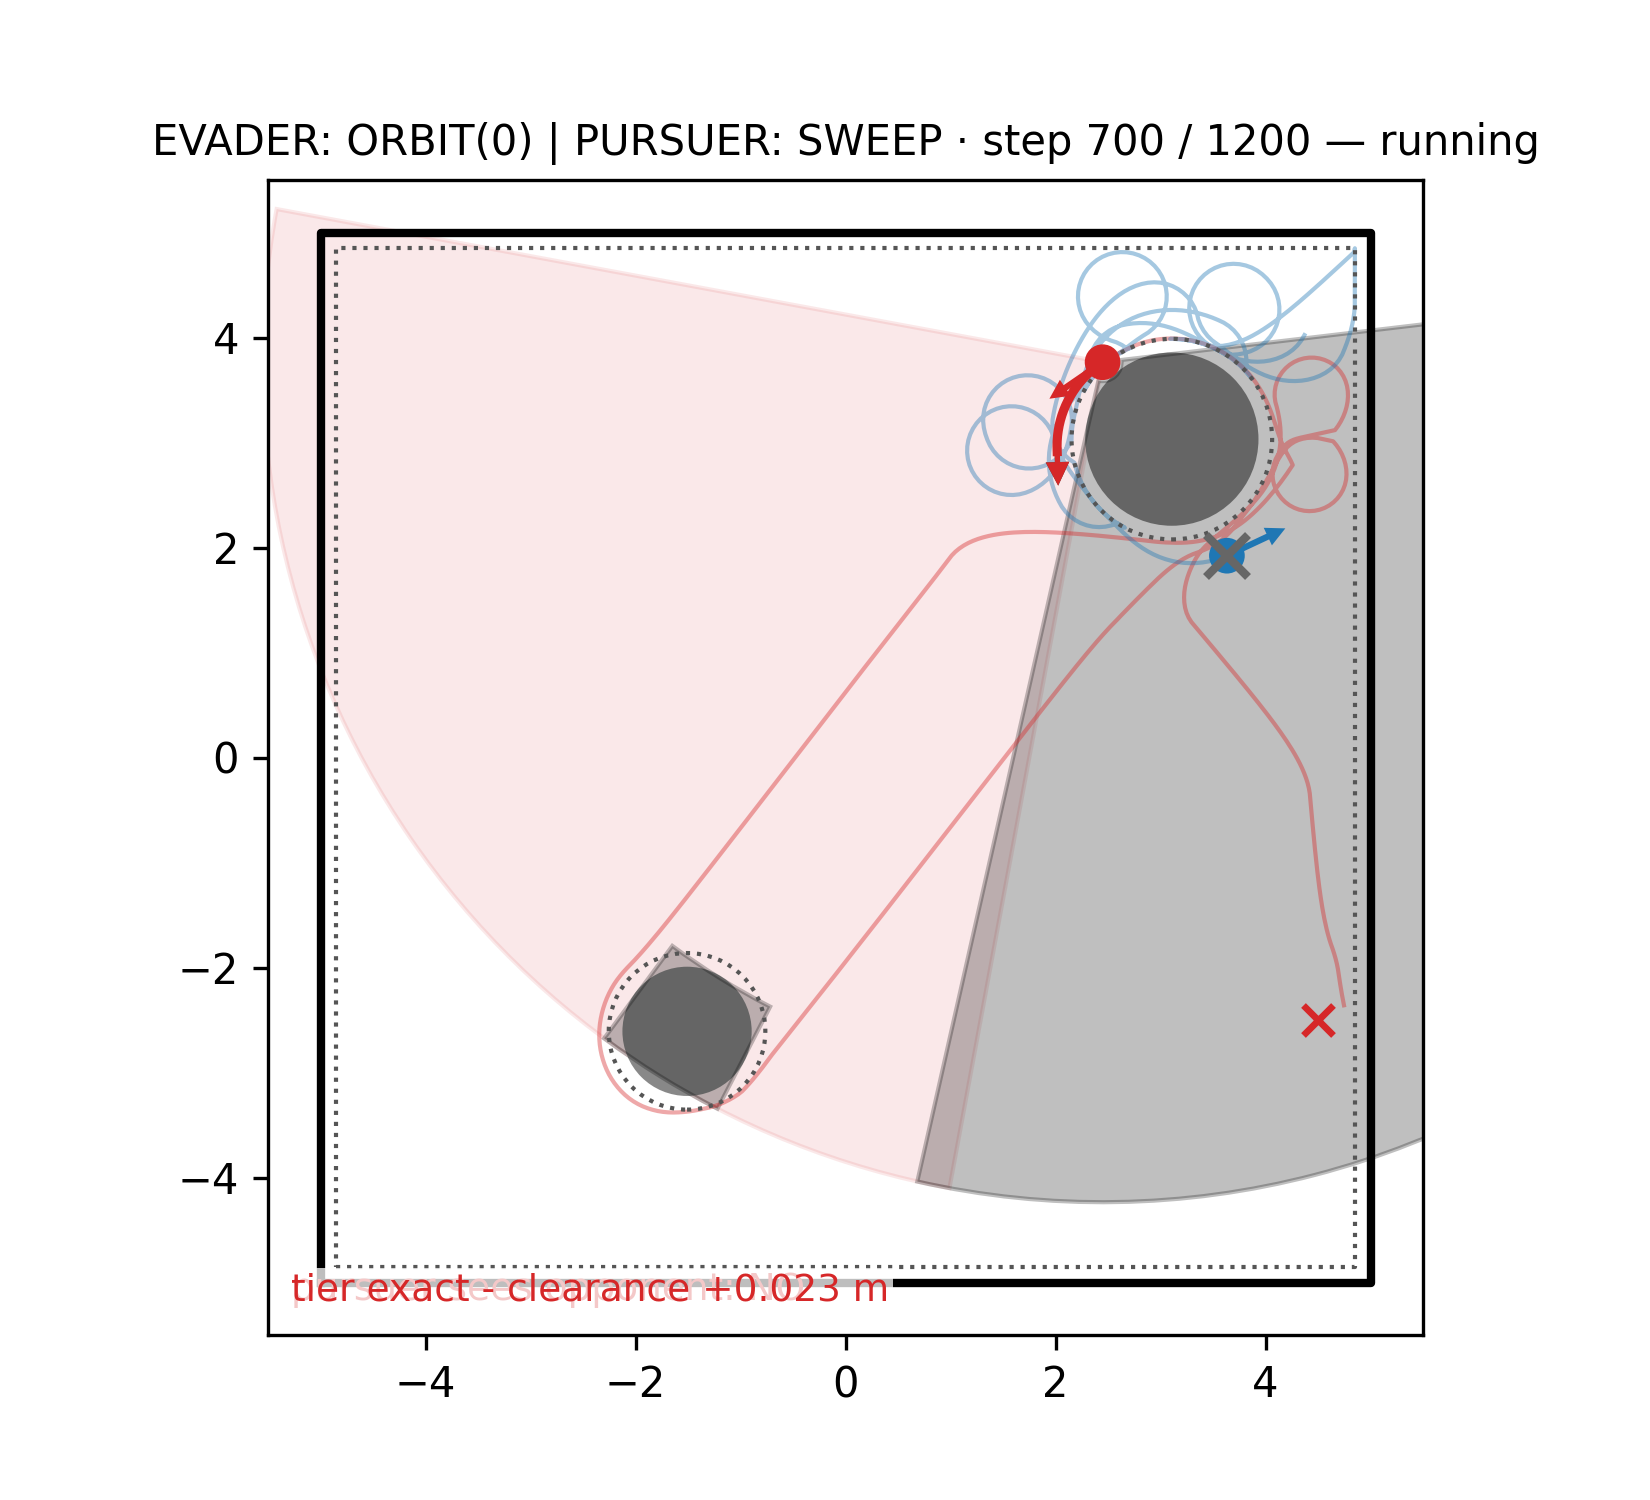
\includegraphics[width=\columnwidth]{figures/episode.png}
\caption{Step 700 of evaluation episode $2\,400\,001$, the retrained selector (red, in \pol{Sweep}) against the learned evader (blue, in \pol{Orbit}), re-rendered from the archived round with the round's own recorder. The evader's loops around the upper obstacle are traced; the pursuer's $90^\circ$ sensing cone is shaded, the cross marks its dead-reckoned target, and the footer reports the filter's tier and the body clearance (0.023\,m). The episode timed out.}
\label{fig:episode}
\end{figure}

\begin{table}[t]
\caption{Capture rate of five frozen pursuers against the learned evader (three seeds), 500 paired episodes per cell. Against the scripted tactical evader the same pursuers captured 0.528, 0.660 and 0.746--0.782.}
\label{tab:evader}
\centering
\small
\begin{tabular}{lccccc}
\toprule
Evader & \pol{Sel}-1 & \pol{Sel}-2 & \pol{Sel}-3 & \pol{Rules} & \pol{Lead} \\
\midrule
\pol{Evs}-1 & 0.130 & 0.136 & 0.128 & 0.110 & 0.086 \\
\pol{Evs}-2 & 0.144 & 0.192 & 0.218 & 0.104 & 0.120 \\
\pol{Evs}-3 & 0.138 & 0.152 & 0.150 & 0.122 & 0.106 \\
\bottomrule
\end{tabular}
\end{table}

\textbf{The pursuer cannot answer within its library.} \pol{Sel-R}, retrained with \pol{Evs}-1 in its opponent mixture, captures $0.11$--$0.17$ against the three learned evaders, no better than the original selector on the same seeds and significantly worse in two pairings ($0.124$ against $0.192$, $p=4\times10^{-4}$; $0.170$ against $0.218$, $p=0.02$), while staying non-inferior against \pol{Greedy} and \pol{Hug} and losing $0.05$--$0.08$ against the tactical evader on two seeds. Its tactic mix shifts towards search (\pol{Sweep} $0.49$--$0.58$ of decisions, \pol{Intercept} $0.24$, \pol{Lead} $0.16$): it looks for the evader more and closes no more often.

\textbf{Meta-game.} Figure~\ref{fig:metagame} reads the $4\times4$ matrix of pursuers \{\pol{Rules}, \pol{Lead}, \pol{Sel}-2, \pol{Sel-R}-1\} against evaders \{\pol{Greedy}, \pol{Hug}, \pol{Tactic}, \pol{Evs}-1\} as a zero-sum game in the capture rate. It has a pure saddle point at (\pol{Sel-R}-1, \pol{Evs}-1) with value $0.138$ and zero duality gap. Exploitability, the value minus a pure policy's worst-case payoff~\cite{wu2026competence}, is $0.028$, $0.052$, $0.002$ and $0$ for the four pursuers: every pursuer in the library is within $0.05$ of the value against the learned evader. For the evaders it is $0.482$, $0.256$, $0.644$ and $0$: the scripted evaders are far from minimax and the learned one is the minimax strategy of this pool. The natural reading, which we registered as the hypothesis of the next round, was that the certified filter sets this value, because the orbit exploits the margin the filter forbids the pursuer to cross.

\begin{figure}[t]
\centering
\includegraphics[width=\columnwidth]{figures/metagame.pdf}
\caption{The $4\times4$ tactic meta-game at speed ratio 1.2 and margin $\delta=0$: pursuer capture rate over 500 paired episodes per cell. The pure saddle point (orange frame) is the retrained selector against the learned evader, value 0.138.}
\label{fig:metagame}
\end{figure}

\subsection{Does the filter set the value?}
\label{sec:res-value}
The margin sweep evaluates four frozen pursuers (\pol{Rules}, \pol{Sel}-2, \pol{Sel-R}-1, \pol{Full}) against four frozen evaders (\pol{Greedy}, \pol{Hug}, \pol{Tactic}, \pol{Evs}-1) under five filter settings: no filter (a pass-through control), and the filter at obstacle margins $\delta\in\{0,0.05,0.10,0.20\}$\,m. The $\delta=0$ cells reproduced the stored records of the earlier rounds bit for bit (all 500 episodes of 12 cells). The pre-registered claim was that removing the filter raises capture against the learned evader for all four pursuers and that the largest margin lowers it for at least three; the refutation sentence stated that the reading ``the filter sets the value'' would be withdrawn where no row rose.

\begin{table}[t]
\caption{Pre-registered tests of the margin sweep: capture rate against the learned evader (500 paired episodes) with no filter, at $\delta=0$ and at $\delta=0.20$\,m, with the exact paired test against $\delta=0$.}
\label{tab:value}
\centering
\small
\begin{tabular}{lccccc}
\toprule
Pursuer & no filter & $p$ & $\delta=0$ & $\delta=0.20$ & $p$ \\
\midrule
\pol{Rules}    & 0.132 & 0.13  & 0.110 & 0.096 & 0.43 \\
\pol{Sel}-2    & 0.170 & 0.046 & 0.136 & 0.088 & 0.001 \\
\pol{Sel-R}-1  & 0.184 & 0.002 & 0.138 & 0.128 & n.s. \\
\pol{Full}     & 0.042 & 0.07  & 0.064 & 0.050 & n.s. \\
\bottomrule
\end{tabular}
\end{table}

\begin{figure*}[t]
\centering
\includegraphics[width=\textwidth]{figures/valuesweep.pdf}
\caption{The margin sweep. (a) Capture rate of four frozen pursuers against the learned evader with no filter and at four obstacle margins; bands are Wilson 95\% intervals over 500 paired episodes. (b) Value of the $4\times4$ capture game at each setting, with the evader in the support of the solution; every setting has a pure saddle point.}
\label{fig:valuesweep}
\end{figure*}

Both hypotheses failed (Table~\ref{tab:value}, Figure~\ref{fig:valuesweep}). Removing the filter raises capture against the learned evader significantly for the two learned pursuers ($+0.034$ and $+0.046$) and not for the rule table, and \pol{Full} falls rather than rises; where the rise holds, the filter's share of the evader's advantage is $0.03$--$0.05$ of capture against an escape rate of $0.82$--$0.86$. The learned evader's obstacle orbit at $\rho=1.2$ beats the unfiltered pursuers on geometry alone. The value of the $4\times4$ game is $0.184$ with no filter, $0.138$ at $\delta=0$, $0.136$ at $0.05$, $0.162$ at $0.10$ and $0.058$ at $0.20$; the pre-stated order (no filter $>$ $\delta=0$ $>$ $\delta=0.20$) holds and the curve is not monotone (the rise at $0.10$ is not significant for any row). Every setting has a pure saddle point, and the pursuer side stays non-exploitable within its library at every setting (exploitability at most $0.054$ for the three library pursuers).

The large margin changes the game in a different way from the one we registered: at $\delta=0.20$ the minimax evader is no longer the learned one but the scripted hugger. A margin of 0.20\,m stops every pursuer from approaching an obstacle-hugging evader at all (capture $0.042$--$0.058$ against $0.38$--$0.39$ at $\delta=0$), and even \pol{Greedy} becomes hard to catch ($0.58$--$0.62$ to $0.11$--$0.12$), while the learned evader's rates barely move. \pol{Full}, the full-state greedy pursuer added to separate information from margin, is the weakest row against every evader at every setting ($0.42$, $0.29$, $0.46$ against the scripted evaders at $\delta=0$, against $0.58$, $0.38$, $0.66$ for \pol{Rules}); the episodes show why: it presses into the obstacle body for a thousand steps while the evader orbits, so it says nothing about information. Without the filter it makes $100\,084$--$285\,595$ contact steps per 500 episodes, and the three library pursuers $15\,505$--$37\,314$; with the filter, at every margin, all 64 cells have zero.

\section{Discussion}
\textbf{What the hierarchy buys.} On the same game, filter, memory features and budget, a learned choice among five closed-loop tactics learns where flat RL collapses and beats a structured law-plus-search learner by $0.05$--$0.47$. The ablations locate the gain: it is not the decision cadence (the cadence-matched flat family is the weaker one), it is mostly the architecture rather than the memory (the no-memory selector is already at or above the fixed law), and it is the selector's choices rather than its library alone (it departs from the rule table over the same library on every opponent and finds \pol{Ambush}). Its limits are the library's limits, which is the legible failure mode a hierarchical design is chosen for: when a slower evader hides behind an obstacle, no tactic reaches it, and adding a plausible one made the pursuer worse.

\textbf{The evader side wins, and quickly.} A single round of learning on the evader side, over five hand-written tactics, finds the obstacle orbit and reduces every pursuer by $0.6$ of capture. The pursuer's retraining changes its mix and not its outcome, and the meta-game confirms that the pursuer's library, not its learning, is binding: every pursuer is within $0.05$ of the value against the learned evader. This is the two-sided version of a known asymmetry of pursuit--evasion among obstacles, with the twist that both players are learned selectors over human-legible tactics, so the equilibrium can be read off the episodes.

\textbf{The filter's share is small, and its margin changes who is minimax.} We registered the hypothesis that the certified filter sets the value, and the sweep refuted it in the form stated. The filter's cost at the default margin is $0.046$ of value, and the learned orbit is minimax with no filter at all; speed ratio, obstacle geometry and the libraries set most of the value. The margin matters in a different way: at $0.20$\,m the pursuer can no longer approach any obstacle-hugging evader, so the solution's support moves from the learned evader to a scripted one and the value drops to $0.058$. The practical reading for safety-filtered competitive systems is that the filter's margin should be reported as a parameter of the game, with the unfiltered value beside it, before any statement about what the filter costs is made. This complements~\cite{wu2026competence}, whose theorem concerns a perfect filter and whose experiments do not vary the filter; here the filter is model-based and its margin is the swept variable.

\textbf{Construct discipline.} Three of the pre-registered hypotheses of this study failed (the per-ratio training, the sixth tactic, and the filter-sets-the-value reading), one gate failed twice (tactic recognition), and the failures changed the design and the claim. Watching the rendered episodes before reading the tables caught two construct errors in the scripted game before any learning round ran (a pursuer pinned at an obstacle by the plain filter, and a search that never found a stationary evader). We report these because the resulting claims are narrower than the ones we set out to make and, we believe, more likely to hold.

\section{Limitations}
\label{sec:limits}
Everything is in simulation, with a known static map and the true pose available to the filter. Each learned arm has three seeds and one budget ($3\times10^{6}$ steps); the learning baselines use the library's default hyper-parameters without a per-baseline search, so a tuned flat learner might do better than reported, although its failure mode (pinning) is the one the filter literature predicts. The two-sided rounds are at a single speed ratio ($1.2$). The margin sweep evaluates \emph{frozen} players across settings, so it measures how fixed policies respond to the filter and not the value of the game with players retrained at each margin; the unfiltered value in particular may understate what an unfiltered pursuer could learn. The meta-game is a $4\times4$ pool, so ``minimax'' is relative to that pool, not to the full game. The scripted evaders and the evader's tactics read the true state while the pursuer's selector is sensing-limited, and two pursuer tactics (\pol{Counter-Orbit} and the facing step of \pol{Ambush}) read the true evader pose while executing although the selector that chooses them does not; the information asymmetry favours the evader and should be kept in mind when reading the two-sided results. Finally, the obstacle's own role was not isolated by removing obstacles; the sweep varied the filter, not the geometry.

\section{Conclusion}
Learned tactic selection over hand-written closed-loop tactics is a workable way to put a reinforcement learner behind a safety filter in a pursuit--evasion game: it beats fixed laws and flat and structured learners, it transfers across speed ratios, and it makes no contact. Applied to both players it converges in one evader step to an obstacle-orbit equilibrium that the pursuer cannot escape within its library. The natural suspicion that the safety filter is what makes that equilibrium favour the evader does not survive a direct test: the filter's share of the value is small, and its margin changes which evader is minimax rather than how strong the learned one is. Future work is the obvious counterpart of the last experiment, players retrained at each margin and a geometry sweep, and a pursuer library with a tactic that can go round an obstacle it cannot see behind.

\section*{Acknowledgment}
\textbf{Generative AI use.} Claude (Anthropic; the Claude Code agent with Claude Opus and Fable 5.x models) was used for experiment code and orchestration, literature search, figure scripts, and drafting and editing of the manuscript. The authors specified the experiments, reviewed every number against the archived records, and take responsibility for the content.
\textbf{Data and code.} The per-cell evaluation records, rendered episodes, pre-registration documents and training and evaluation code will be released at the repository given at camera-ready.
\textbf{Conflicts of interest.} None declared.

\bibliographystyle{IEEEtran}
\bibliography{references}

\end{document}
